% !TEX program = pdflatex
\documentclass[11pt,oneside,openany]{book}

\usepackage[T1]{fontenc}
\usepackage[utf8]{inputenc}
\usepackage{lmodern}
\usepackage[letterpaper,margin=1in,headheight=15pt]{geometry}
\usepackage{microtype}
\usepackage{amsmath,amssymb}
\usepackage{booktabs,longtable,tabularx,array}
\usepackage{xcolor}
\usepackage{listings}
\usepackage{enumitem}
\usepackage{fancyhdr}
\usepackage{graphicx}
\usepackage{tikz}
\usetikzlibrary{arrows.meta,positioning,shapes.geometric,fit}
\usepackage{makeidx}
\usepackage{url}
\usepackage[hidelinks]{hyperref}
\usepackage{bookmark}

\makeindex
\setcounter{secnumdepth}{3}
\setcounter{tocdepth}{2}
\renewcommand{\arraystretch}{1.18}
\newcolumntype{Y}{>{\raggedright\arraybackslash}X}
\newcommand{\projectroot}{\path{/home/justneeraj/Documents/MS_sem3/GRAD_PROJECT}}
\newcommand{\term}[1]{\textbf{#1}\index{#1}}
\newcommand{\file}[1]{\path{#1}}
\newcommand{\state}[1]{\texttt{#1}}

\definecolor{codebg}{RGB}{246,248,250}
\definecolor{codeframe}{RGB}{208,215,222}
\definecolor{keyword}{RGB}{0,75,135}
\definecolor{comment}{RGB}{80,110,80}
\lstdefinestyle{ee616}{
  backgroundcolor=\color{codebg},
  frame=single,
  rulecolor=\color{codeframe},
  basicstyle=\ttfamily\small,
  keywordstyle=\color{keyword}\bfseries,
  commentstyle=\color{comment},
  breaklines=true,
  breakatwhitespace=false,
  columns=fullflexible,
  keepspaces=true,
  showstringspaces=false,
  upquote=true
}
\lstset{style=ee616}

\pagestyle{fancy}
\fancyhf{}
\fancyhead[L]{EE 616 Project Handbook}
\fancyhead[R]{Neeraj Kumar Kanchani}
\fancyfoot[C]{\thepage}

\hypersetup{
  pdftitle={Vision-Based Predecessor-Following Warehouse Convoys: Project Handbook and Simulation User Guide},
  pdfauthor={Neeraj Kumar Kanchani},
  pdfsubject={EE 616 ROS 2 and Gazebo project handbook},
  pdfkeywords={ROS 2, Gazebo, leader follower, predecessor following, YOLOv8n, EKF, warehouse robotics}
}

\title{\Huge Vision-Based Predecessor-Following\\Warehouse Convoys\\[0.4em]
\Large Project Handbook, Simulation User Guide,\\and Evidence Reference}
\author{\Large Neeraj Kumar Kanchani\\[0.7em]
EE 616-57, Section 9189, Four Credits\\
Faculty Reviewer: Professor Masudul Imtiaz}
\date{Frozen Gate 7 edition\\September 30, 2026}

\begin{document}
\frontmatter
\hypersetup{pageanchor=false}
\maketitle
\clearpage
\hypersetup{pageanchor=true}

\chapter*{Document purpose}
\addcontentsline{toc}{chapter}{Document purpose}

This handbook explains the complete software and simulation project in a form that can be studied, operated, changed, and defended. It is not the final faculty report. The faculty report remains the project owner's own writing. The handbook is a technical reference for learning the system, reproducing the experiments, understanding every recorded metric, and planning later revisions.

The implemented system is a ROS~2 Jazzy and Gazebo Harmonic simulation of one route-owning leader and independently driven predecessor-following robots. Every follower uses a forward RGB camera and local wheel odometry. The accepted pipeline contains YOLOv8n target detection, monocular range and bearing, a relative-state extended Kalman filter, bounded formation control, and the states \state{TRACK}, \state{PREDICT}, and \state{SAFE\_STOP}. Gazebo pose truth is restricted to evaluation.

This document deliberately distinguishes four levels of evidence:
\begin{enumerate}
  \item mathematical definitions and software design;
  \item deterministic toy-model results;
  \item ROS~2 and Gazebo simulation results on one laptop; and
  \item physical or industrial claims, which have not been demonstrated.
\end{enumerate}

\chapter*{Assistance and responsibility statement}
\addcontentsline{toc}{chapter}{Assistance and responsibility statement}

An AI assistant supported code development, experiment organization, documentation structure, editing, and generation of this handbook. Neeraj Kumar Kanchani is responsible for reviewing the source, verifying the evidence, understanding the equations and commands, and deciding what to submit or present. This handbook must not be used to conceal AI assistance or to claim work that the project owner cannot explain.

\chapter*{How to use this book}
\addcontentsline{toc}{chapter}{How to use this book}

Read Part~I before explaining the project to another person. Read Part~II when studying the algorithms. Use Part~III while operating the software. Use Part~IV before changing parameters or designing a new experiment. Use Part~V when interpreting results. The appendices provide command, topic, parameter, definition, and oral-examination references.

Commands assume that the current directory is the single authorized workspace:
\begin{center}
\projectroot
\end{center}
Do not create a second project workspace. Generated ROS directories remain inside \file{work/ros2_ws/}.

\tableofcontents
\listoftables
\listoffigures

\mainmatter

\part{Problem, Scope, and Engineering Foundations}

\chapter{The core problem}
\index{warehouse material transport}\index{leader--follower control}\index{project contribution}

\section{Application problem}

The application is warehouse material transport. A leader owns a route. One or more independently driven carts follow it. The carts are not mechanically connected. Follower~1 observes the leader, Follower~2 observes Follower~1, and each later follower observes its immediate predecessor. This is a \term{predecessor-following topology}.

The technical problem is not simply ``make robots follow.'' The measurable question is:

\begin{quote}
How accurately and reliably can a resource-constrained follower maintain a requested predecessor-relative gap using a forward RGB camera and local wheel odometry during changes in range, bearing, route curvature, target visibility, and bounded disturbances?
\end{quote}

The follower does not receive the leader's global route, global pose, or Gazebo pose. It must infer relative geometry from the image and combine that measurement with its own motion estimate.

\section{Why the problem is difficult}

Five coupled effects make the problem interesting.
\begin{enumerate}
  \item A monocular image does not directly contain metric depth. Metric range requires known geometry or learned depth cues.
  \item A detector can miss, clip, or mislocalize a target. Image errors become range and bearing errors.
  \item A controller changes the camera viewpoint, so perception and motion form a closed loop.
  \item Temporary visual loss requires a defined recovery policy. Continuing indefinitely is unsafe; stopping immediately for every missed frame can be impractical.
  \item In a chain, the motion error of an early follower changes the target motion seen by the next follower. Error can grow, decrease, or change with the scenario.
\end{enumerate}

\section{Implemented solution}

The implemented follower executes this sequence:
\begin{enumerate}
  \item receive a 640 by 480 RGB image;
  \item detect a known red rear target with a trained YOLOv8n model;
  \item convert its bounding box to relative range and bearing;
  \item combine the measurement with local wheel odometry in a four-state EKF;
  \item calculate bounded linear and angular commands;
  \item select \state{TRACK}, \state{PREDICT}, or \state{SAFE\_STOP} from measurement age;
  \item publish commands and synchronized diagnostic topics; and
  \item log performance using a separate evaluation-only process.
\end{enumerate}

\section{Why this project is worth doing}

The project does not claim invention of leader--follower control, camera following, visual markers, monocular range estimation, or Kalman filtering. Related systems already exist \cite{platoon2017,ibvs2020,fisheye2023,range2024,marker2025,platooning2025}. The defensible contribution is the implementation and evaluation of one constrained architecture:
\begin{itemize}
  \item warehouse-focused predecessor following;
  \item independently driven followers;
  \item forward RGB and local odometry at each follower;
  \item explicit visual-loss states;
  \item evaluation-only ground truth;
  \item pair-first and incremental-chain validation;
  \item rearward error measurements;
  \item controlled visual-loss and command-bias tests; and
  \item timing and resource measurements on a 4~GiB laptop GPU.
\end{itemize}

This makes the project useful as a systems-integration and experimental-method study. Its strength is not a first-ever algorithm. Its strength is traceable engineering evidence and clear limits.

\chapter{System boundary and claims}
\index{claim boundary}\index{safety boundary}\index{production readiness}

\section{Inside the research system}

The research system includes leader route generation, follower camera sensing, predecessor detection, relative geometry, estimation, formation control, supervision, ROS~2 communication, Gazebo dynamics, logging, and offline evaluation.

\section{Outside the research system}

The following items are outside the demonstrated scope:
\begin{itemize}
  \item physical robots;
  \item safety-rated LiDAR or person detection;
  \item certified emergency stopping;
  \item warehouse fleet management;
  \item wireless network delay and packet loss;
  \item physical wheel slip and detailed motor dynamics;
  \item industrial commissioning and standards compliance; and
  \item production readiness.
\end{itemize}

\section{Ground-truth firewall}

\term{Ground truth} is the simulator's direct knowledge of model pose. It is useful for calculating error but unavailable to a camera-only physical follower. Therefore, Gazebo pose truth may be consumed only by \file{ee616_evaluation}. It must never enter \file{ee616_perception}, the EKF, the supervisor, the controller, or the disturbance proxy.

\begin{figure}[htbp]
\centering
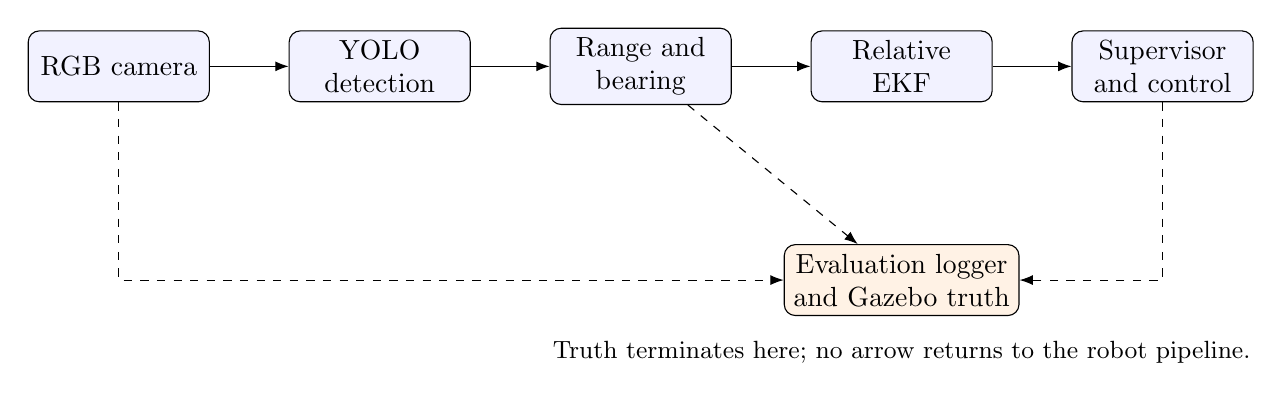
\begin{tikzpicture}[node distance=8mm and 10mm,>=Latex,
  box/.style={draw,rounded corners,align=center,minimum height=9mm,minimum width=23mm,fill=blue!5},
  eval/.style={draw,rounded corners,align=center,minimum height=9mm,fill=orange!10}]
\node[box] (cam) {RGB camera};
\node[box,right=of cam] (det) {YOLO\\detection};
\node[box,right=of det] (geom) {Range and\\bearing};
\node[box,right=of geom] (ekf) {Relative\\EKF};
\node[box,right=of ekf] (sup) {Supervisor\\and control};
\draw[->] (cam)--(det); \draw[->] (det)--(geom); \draw[->] (geom)--(ekf); \draw[->] (ekf)--(sup);
\node[eval,below=18mm of ekf] (truth) {Evaluation logger\\and Gazebo truth};
\draw[dashed,->] (cam) |- (truth);
\draw[dashed,->] (geom) -- (truth);
\draw[dashed,->] (sup) |- (truth);
\node[below=2mm of truth,align=center,font=\small] {Truth terminates here; no arrow returns to the robot pipeline.};
\end{tikzpicture}
\caption{Runtime information boundary. Dashed arrows are logging paths.}
\label{fig:boundary}
\end{figure}

\section{Safe language}

Use statements such as ``the evaluator recorded zero collision samples under the defined simulation check.'' Do not replace that statement with ``the system is collision-free'' or ``the robots are safe.'' A finite simulator run cannot establish general safety.

\chapter{Essential robotics definitions}
\index{pose}\index{transform}\index{open loop}\index{closed loop}\index{determinism}

\section{Pose, frame, and transform}

A \term{pose} contains position and orientation. In the planar experiments, a pose is $(x,y,\psi)$, where $\psi$ is yaw. A \term{coordinate frame} defines the origin and axes used to express a quantity. A \term{transform} converts a point or pose between frames.

The follower camera frame is attached to the follower. Relative range and bearing are expressed from that camera viewpoint. Odometry is local motion information published in the robot's odometry frame. Gazebo's world frame is evaluation-only.

\section{Range and bearing}

\term{Range} is the straight-line planar distance from camera to target. \term{Bearing} is the horizontal target angle relative to the camera's forward axis. In this implementation, a target left of image center produces positive bearing because the calculation uses $(c_x-u)/f$.

\section{Odometry}

\term{Wheel odometry} estimates motion from wheel movement. The controller uses local forward speed and yaw rate from the ROS \file{nav_msgs/Odometry} message. Simulation odometry is cleaner than physical wheel odometry; the current evidence does not include real encoder error or slip.

\section{Open loop and closed loop}

An \term{open-loop} measurement test moves or places a target but does not let the detector control the robot. A \term{closed-loop} experiment feeds the measurement through estimation and control so that output motion changes later measurements. Gate~2 is measurement-only. Gates~3--6 are closed loop.

\section{Determinism and repeatability}

A deterministic configuration should produce equivalent behavior when initial conditions, software, and hardware scheduling are controlled. Exact floating-point samples can still vary because ROS callbacks and GPU execution are scheduled concurrently. The project therefore uses repeated trials and bounded acceptance criteria rather than requiring byte-identical dynamic CSV files.

\part{Implemented Architecture and Algorithms}

\chapter{Robot topology and ROS namespaces}
\index{ROS 2}\index{namespace}\index{topic}\index{predecessor following}

\section{Chain structure}

The leader owns the route. It publishes its own motion command. Each follower runs a copy of the same perception and control stack in an isolated namespace.

\begin{figure}[htbp]
\centering
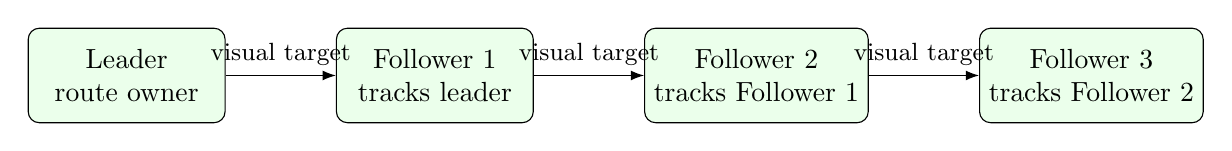
\begin{tikzpicture}[>=Latex,node distance=14mm,
robot/.style={draw,rounded corners,minimum width=25mm,minimum height=12mm,align=center,fill=green!8}]
\node[robot] (l) {Leader\\route owner};
\node[robot,right=of l] (f1) {Follower 1\\tracks leader};
\node[robot,right=of f1] (f2) {Follower 2\\tracks Follower 1};
\node[robot,right=of f2] (f3) {Follower 3\\tracks Follower 2};
\draw[->] (l)--node[above,font=\small]{visual target}(f1);
\draw[->] (f1)--node[above,font=\small]{visual target}(f2);
\draw[->] (f2)--node[above,font=\small]{visual target}(f3);
\end{tikzpicture}
\caption{Implemented maximum convoy used in the accepted demonstration.}
\end{figure}

\section{Namespace rule}

Namespaces prevent similarly named topics from colliding. The accepted runtime uses \file{/leader}, \file{/follower_1}, \file{/follower_2}, and \file{/follower_3}. For example, \file{/follower_2/odom} is not the same topic as \file{/follower_3/odom}.

\section{Package responsibilities}

\begin{longtable}{@{}p{0.23\textwidth}p{0.68\textwidth}@{}}
\toprule
Package & Implemented responsibility \\
\midrule
\endhead
\file{ee616_bringup} & Namespace and camera transport probes for environment validation. \\
\file{ee616_simulation} & Gazebo worlds, generated robots, scenario templates, bridges, and disturbance proxy. \\
\file{ee616_perception} & Deterministic red-target baseline, YOLOv8n target detection, range/bearing conversion, and inference diagnostics. \\
\file{ee616_control} & Relative EKF, measurement-age supervisor, bounded follower controller, and deterministic leader route. \\
\file{ee616_evaluation} & Measurement, pair, chain, disturbance, timing, plotting, and summary tools. It alone may read Gazebo truth. \\
\bottomrule
\end{longtable}

Estimation and supervision are implemented inside \file{ee616_control}; there are not separate \file{ee616_estimation} and \file{ee616_supervisor} packages in the frozen system.

\chapter{Gazebo robot and sensor model}
\index{Gazebo}\index{differential drive}\index{camera model}\index{visual target}

\section{Robot body}

Each generated robot has a rectangular base, two driven wheels, and two low-friction caster collision shapes. The body mass is 8.0~kg, each wheel mass is 0.5~kg, wheel radius is 0.10~m, and wheel separation is 0.46~m. Gazebo's differential-drive system consumes a namespaced \file{cmd_vel} topic and publishes odometry at 30~Hz.

These values form a simplified simulation model. They are not measurements from a selected physical cart.

\section{Camera}

Each follower has a front camera mounted 0.28~m forward and 0.43~m above the base-link origin. It requests 640 by 480 RGB images at 15~Hz, with a 70-degree horizontal field of view and 0.1--30~m clipping range.

\section{Rear visual target}

Every robot that can be observed from behind carries a red rectangular target. The target geometry is 0.08~m thick, 0.70~m wide, and 0.90~m high. The range equation assumes the 0.90~m height is known.

\section{Physics and rendering}

The generated pair and chain worlds use a 0.005~s maximum physics step and a requested real-time factor of 1.0. Shadows are disabled. Recorded experiments are headless. The system reports EGL and rendering fallback warnings on the laptop, so GPU passthrough is verified but accelerated Gazebo rendering is not claimed.

\chapter{Visual perception}
\index{YOLOv8n}\index{RGB/BGR contract}\index{confidence threshold}\index{failed experiments}

\section{Why use a known target}

A known rear target makes the first metric range calculation identifiable. The project can separate detection error from the geometry equation. This is a valid engineering baseline, but it assumes the predecessor has a visible target of known dimensions.

\section{YOLOv8n input contract}

The ROS node converts \file{sensor_msgs/Image} to an RGB NumPy array. Ultralytics' array interface is supplied a contiguous BGR array, so the implementation reverses the color channels before inference. An earlier RGB/BGR mismatch was one reason a prior detector failed.

The accepted v3 configuration is:
\begin{longtable}{@{}p{0.34\textwidth}p{0.20\textwidth}p{0.37\textwidth}@{}}
\toprule
Parameter & Value & Meaning \\
\midrule
\endhead
\file{weights_path} & v3 checkpoint & Accepted trained model. \\
\file{class_id} & 0 & The only class is \file{predecessor_target}. \\
\file{confidence} & 0.40 & Validation-selected minimum box confidence. \\
\file{iou} & 0.45 & Non-maximum-suppression overlap setting. \\
\file{image_size} & 640 & YOLO inference size. \\
\file{device} & \file{0} & First CUDA device. \\
\file{range_scale} & 0.9903208 & Validation-only linear calibration scale. \\
\file{range_offset_m} & 0.1042198 & Validation-only linear calibration offset in metres. \\
\bottomrule
\end{longtable}

\section{Detection selection}

The detector filters predictions to class~0 and selects the highest-confidence remaining box. If no valid box exists, it publishes an invalid measurement using NaN range and bearing and a validity field of zero. A valid measurement has vector fields $(r,\beta,1)$.

\section{Why the failed detectors matter}

The v1 detector reached only 79.6\% valid full-visible measurements and 0.505~m range RMSE. The v2 corrective detector produced zero valid detections on its unchanged final scenes. Both remain recorded failures. The synchronized v3 dataset corrected the image contract and stale-frame label problem and passed a new sealed two-scene gate. Preserving this sequence demonstrates diagnosis rather than selective reporting.

\chapter{Monocular range and bearing geometry}
\index{monocular geometry}\index{focal length}\index{field of view}\index{range calibration}

\section{Focal length from horizontal field of view}

For image width $W$ and horizontal field of view $\phi$, the focal length in pixels is
\begin{equation}
f_x = \frac{W}{2\tan(\phi/2)}.
\end{equation}
The project uses $W=640$ and $\phi=1.2217304764$~rad, which is 70 degrees.

\section{Bearing}

Let $u$ be the detected box center and $c_x=(W-1)/2$ the principal point. The implementation calculates
\begin{equation}
\hat\beta=\tan^{-1}\left(\frac{c_x-u}{f_x}\right).
\end{equation}
This sign convention treats image-left as positive bearing.

\section{Range}

Let $H$ be known target height and $h$ detected pixel height. The forward optical depth is
\begin{equation}
\hat z=\frac{f_xH}{h}.
\end{equation}
Because the project reports planar line-of-sight range rather than optical-axis depth, it calculates
\begin{equation}
\hat r_{\mathrm{raw}}=\frac{\hat z}{\cos\hat\beta}.
\end{equation}
The accepted calibration is
\begin{equation}
\hat r=0.9903207646\,\hat r_{\mathrm{raw}}+0.1042197665.
\end{equation}

\section{Failure mechanisms}

Range error grows when the target is small, clipped, tilted, partly hidden, or localized with the wrong vertical bounds. Calibration cannot repair a completely missed or incorrect detection. It also must not be fit using final test scenes.

\chapter{Relative-state extended Kalman filter}
\index{extended Kalman filter}\index{EKF|see{extended Kalman filter}}\index{covariance}\index{innovation}

\section{State vector}

The implemented EKF state is
\begin{equation}
\mathbf{x}=\begin{bmatrix}r & \beta & \dot r & \dot\beta\end{bmatrix}^{\mathsf T}.
\end{equation}
It represents relative range, relative bearing, and two predecessor-driven rate terms. It is not a global pose filter.

\section{Prediction model}

Let the follower's measured forward speed be $v_f$, yaw rate be $\omega_f$, and step be $\Delta t$. The nonlinear prediction is
\begin{align}
r^+ &= r+(\dot r-v_f\cos\beta)\Delta t,\\
\beta^+ &= \operatorname{wrap}\left[\beta+\left(\dot\beta+\frac{v_f\sin\beta}{r}-\omega_f\right)\Delta t\right],\\
\dot r^+ &= \dot r,\\
\dot\beta^+ &= \dot\beta.
\end{align}
The implementation clamps $\Delta t$ to at most 0.20~s and range to at least 0.05~m. It propagates covariance with the Jacobian $\mathbf F$ and additive process covariance $\mathbf Q$.

\section{Measurement update}

The measurement is
\begin{equation}
\mathbf z=\begin{bmatrix}r_m & \beta_m\end{bmatrix}^{\mathsf T},\qquad
\mathbf H=\begin{bmatrix}1&0&0&0\\0&1&0&0\end{bmatrix}.
\end{equation}
The bearing innovation is angle-wrapped. The measurement covariance uses standard deviations of 0.04~m and 0.5 degrees. The Kalman gain is
\begin{equation}
\mathbf K=\mathbf P^-\mathbf H^{\mathsf T}
(\mathbf H\mathbf P^-\mathbf H^{\mathsf T}+\mathbf R)^{-1},
\end{equation}
The source code uses this same matrix expression.

\section{Initialization}

The first valid measurement initializes range and bearing. Both rate terms start at zero. Before initialization, the supervisor commands \state{SAFE\_STOP}.

\section{Interpretation limit}

The filter is an engineering relative-state estimator. It has not been proven observable for all routes, and its covariance consistency has not been tested with normalized innovation statistics. Physical odometry drift and wheel slip remain unverified.

\chapter{Bounded control and visual-loss supervision}
\index{formation control}\index{command saturation}\index{TRACK}\index{PREDICT}\index{SAFE STOP}

\section{Control law}

The requested range is $r_d=1.50$~m. The unsaturated commands are
\begin{align}
v_c &= K_{\dot r}\dot r+K_r(r-r_d),\\
\omega_c &= K_\beta\beta+K_{\dot\beta}\dot\beta.
\end{align}
The accepted gains are $K_r=0.85$, $K_{\dot r}=0.85$, $K_\beta=1.80$, and $K_{\dot\beta}=0.20$. Commands are bounded as
\begin{align}
v &= \operatorname{clip}(v_c,0,0.60)\ \mathrm{m/s},\\
\omega &= \operatorname{clip}(\omega_c,-0.80,0.80)\ \mathrm{rad/s}.
\end{align}

The lower linear bound is zero. Therefore, the follower does not reverse to correct a short gap. This explains the roughly 0.12~m short-gap undershoot retained in stopped-leader pair tests.

\section{Supervisor states}

Let $a$ be the age of the most recent valid measurement.
\begin{longtable}{@{}p{0.20\textwidth}p{0.24\textwidth}p{0.47\textwidth}@{}}
\toprule
State & Condition & Action \\
\midrule
\endhead
\state{TRACK} & $a\leq0.20$~s & Use EKF state and full bounded controller. \\
\state{PREDICT} & $0.20<a\leq0.75$~s & Use EKF prediction and multiply linear speed by 0.55. \\
\state{SAFE\_STOP} & $a>0.75$~s or filter uninitialized & Publish zero linear and angular command. \\
\bottomrule
\end{longtable}

\begin{figure}[htbp]
\centering
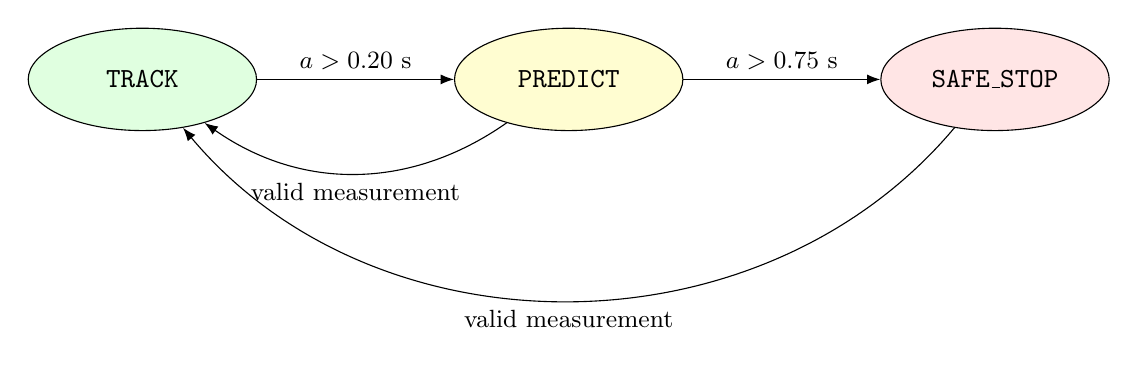
\begin{tikzpicture}[>=Latex,node distance=25mm,
s/.style={draw,ellipse,minimum width=29mm,minimum height=13mm,align=center}]
\node[s,fill=green!12] (track) {\state{TRACK}};
\node[s,fill=yellow!18,right=of track] (predict) {\state{PREDICT}};
\node[s,fill=red!10,right=of predict] (stop) {\state{SAFE\_STOP}};
\draw[->] (track) -- node[above,font=\small]{$a>0.20$ s} (predict);
\draw[->] (predict) -- node[above,font=\small]{$a>0.75$ s} (stop);
\draw[->,bend left=35] (predict) to node[below,font=\small]{valid measurement} (track);
\draw[->,bend left=50] (stop) to node[below,font=\small]{valid measurement} (track);
\end{tikzpicture}
\caption{Implemented measurement-age supervisor.}
\end{figure}

\section{What \state{SAFE\_STOP} means}

It means the software publishes zero commanded velocity after prolonged visual loss. It does not prove a physical stopping distance, emergency-stop integrity, obstacle detection, or functional safety.

\chapter{Leader routes and disturbances}
\index{leader route}\index{occlusion}\index{RGB blackout}\index{actuator bias}\index{disturbance}

\section{Deterministic leader}

The leader is a controlled experimental input. It is not an autonomous warehouse navigator in the frozen gates. Its ordinary linear command is 0.35~m/s. The gradual turn uses 0.12~rad/s; the sharp turn uses 0.18~rad/s.

\section{Nominal profiles}

The \file{straight} profile moves for 16~s after settling. The \file{turn} profile moves straight for 5~s, turns for 8~s, and returns to straight motion for 5~s.

\section{Controlled disturbances}

Gate~5 uses five pair scenarios and one combined chain scenario:
\begin{itemize}
  \item sharp turn;
  \item 0.5~s full-frame RGB blackout;
  \item 1.3~s full-frame RGB blackout;
  \item four-second leader stop;
  \item 0.5~s post-controller angular-command bias of 0.15~rad/s; and
  \item a combined route applying the events to Follower~2 in a three-follower chain.
\end{itemize}

The image blackout replaces all image bytes with zero. It is not a physical object moving between robots. The actuator bias changes the command after the controller and clamps it to the normal limits. It is not wheel slip.

\part{Environment, Setup, and Daily Operation}

\chapter{Canonical software environment}
\index{Docker}\index{Ubuntu Noble}\index{ROS 2!Jazzy}\index{Gazebo!Harmonic}\index{GPU}

\section{Why the project uses Docker}

The laptop host runs Ubuntu 26.04.1 and contains only a partial ROS~2 Lyrical installation. The project does not use that host installation. The canonical container is based on Ubuntu 24.04 Noble with ROS~2 Jazzy, Gazebo Harmonic, \file{ros_gz}, Python, PyTorch, and Ultralytics.

Docker reduces host-version coupling. It does not make an experiment automatically reproducible; configurations, seeds, weights, versions, and outputs still must be recorded.

\section{Target laptop}

The target is an MSI Katana GF66 12UD with an Intel Core i5-12450H, 16~GB RAM, and NVIDIA RTX 3050~Ti Laptop GPU with 4~GB VRAM. The system must be designed for that resource limit.

\section{Container services}

\begin{longtable}{@{}p{0.18\textwidth}p{0.72\textwidth}@{}}
\toprule
Service & Purpose \\
\midrule
\endhead
\file{dev} & Interactive CPU/software-rendering development shell. \\
\file{check} & Automated environment validation. \\
\file{gpu} & GPU-enabled shell and experiment runner with NVIDIA compute, graphics, and utility capabilities. \\
\bottomrule
\end{longtable}

The project uses host networking, shared IPC, a 1~GB shared-memory allocation, ROS domain ID~57, Fast DDS, and Gazebo partition \file{ee616}.

\chapter{First-time setup}
\index{installation}\index{VS Code}\index{Dev Container}\index{NVIDIA Container Toolkit}

\section{Open the only authorized workspace}

\begin{lstlisting}[language=bash]
cd /home/justneeraj/Documents/MS_sem3/GRAD_PROJECT
git status --short --branch
\end{lstlisting}

Do not initialize another repository or copy the project to a second development folder.

\section{Build and validate the container}

\begin{lstlisting}[language=bash]
make container-config
make container-build
make environment-check
make environment-check-gpu
\end{lstlisting}

The final command requires the NVIDIA Container Toolkit. Docker group membership is root-equivalent access; it is a host security decision, not a project convenience to apply silently.

\section{Open VS Code}

Start VS Code from the logged-in graphical desktop terminal:
\begin{lstlisting}[language=bash]
cd /home/justneeraj/Documents/MS_sem3/GRAD_PROJECT
code .
\end{lstlisting}
Choose \textbf{Dev Containers: Reopen in Container}. The container opens \file{/workspace}, which is a bind mount of the same authorized host directory, not a second project copy.

\section{Verify the shell}

Inside the container:
\begin{lstlisting}[language=bash]
echo "$ROS_DISTRO"
ros2 --help
gz sim --version
cd /workspace/work/ros2_ws
colcon build --symlink-install
source install/setup.bash
ros2 pkg list | grep ee616
\end{lstlisting}

\chapter{Daily development workflow}
\index{colcon}\index{ros2 command}\index{gz command}\index{shutdown}

\section{Recommended sequence}

\begin{enumerate}
  \item Check Git status and preserve unrelated changes.
  \item Open the Dev Container.
  \item Run \textbf{EE616: Build ROS workspace}.
  \item Run \textbf{EE616: Test ROS workspace}.
  \item Launch one selected scenario or open the learning shell.
  \item Inspect topics and nodes before changing code.
  \item Stop the simulation cleanly.
  \item Record what changed, why it changed, and which evidence was regenerated.
\end{enumerate}

\section{ROS inspection commands}

\begin{lstlisting}[language=bash]
ros2 node list
ros2 topic list
ros2 topic info /follower_1/camera/image
ros2 topic hz /follower_1/camera/image
ros2 topic echo --once /follower_1/control/state
ros2 node info /follower_1/follower_controller
gz topic -l
\end{lstlisting}

A listed topic proves only discovery. Use \file{topic info}, \file{topic hz}, message inspection, timestamps, and an experiment-specific validator to evaluate data quality.

\section{Stopping processes}

Use Ctrl+C in the active launch terminal. If the terminal was closed, use the VS Code stop task or:
\begin{lstlisting}[language=bash]
bash infrastructure/dev/stop_simulation.sh
\end{lstlisting}

\chapter{Using Gazebo interactively}
\index{Gazebo!GUI}\index{scenario template}\index{AWS warehouse}

\section{Open the playground}

From the host desktop session:
\begin{lstlisting}[language=bash]
make gazebo-gui
\end{lstlisting}
The playground contains a floor, six shelf blocks, a fixed camera, and a visual target. It is for learning. It is not a closed-loop performance experiment.

\section{GUI operations}

Select an entity in the Entity Tree, inspect components, use translation and rotation controls, pause simulation before precise edits, and display collision geometry when studying contact shapes. A GUI-only change is not reproducible until it is saved as source configuration.

\section{Controlled scenario templates}

Run a template with:
\begin{lstlisting}[language=bash]
make scenario-gui SCENARIO=straight_aisle
make scenario-gui SCENARIO=partial_occlusion
make scenario-validate
\end{lstlisting}

The five development templates are camera calibration, straight aisle, right-angle turn, narrow aisle, and partial occlusion. They share a deterministic seed, camera interface, target geometry, and base lighting.

\section{AWS warehouse}

The pinned AWS no-roof world is an optional visual and resource stress test:
\begin{lstlisting}[language=bash]
make aws-warehouse-gui
make aws-benchmark
\end{lstlisting}
It does not contain the accepted follower-control experiment and must not be used as evidence of control accuracy.

\chapter{Running the frozen experiments}
\index{experiment runner}\index{environment gate}\index{pair gate}\index{chain gate}\index{disturbance gate}\index{timing gate}

\section{Important overwrite warning}

The experiment runners write into fixed result directories. Running them again can replace frozen local evidence. Verify the Gate~7 package first, and create a newly named experiment protocol and result directory for exploratory changes.

\section{Environment gate}

\begin{lstlisting}[language=bash]
make environment-check-gpu
\end{lstlisting}
This builds and tests packages, checks namespaces, transports camera data, and records machine information. It is not a follower-performance gate.

\section{Camera measurement gates}

The deterministic camera measurement runner is:
\begin{lstlisting}[language=bash]
docker compose --profile gpu run --rm gpu \
  bash /workspace/work/ros2_ws/scripts/run_camera_measurement_gate.sh
\end{lstlisting}
The accepted learned detector runner is:
\begin{lstlisting}[language=bash]
docker compose --profile gpu run --rm gpu \
  bash /workspace/work/ros2_ws/scripts/run_yolo_measurement_gate_v3.sh
\end{lstlisting}

\section{Nominal pair}

\begin{lstlisting}[language=bash]
make pair-gate
\end{lstlisting}
This runs three straight and three gradual-turn trials.

\section{Incremental chain}

\begin{lstlisting}[language=bash]
make chain-gate
\end{lstlisting}
The script requires all two-follower trials to pass before launching three followers.

\section{Controlled disturbances}

\begin{lstlisting}[language=bash]
make disturbance-gate
\end{lstlisting}
The script requires all fifteen pair trials to pass before three combined chain trials.

\section{Timing and resources}

\begin{lstlisting}[language=bash]
make timing-gate
\end{lstlisting}
This repeats the accepted combined scenario three times and adds an observer-only timing process plus 0.25~s resource sampling.

\section{Run one launch manually}

Inside \file{make gpu-shell}:
\begin{lstlisting}[language=bash]
source /opt/ros/jazzy/setup.bash
cd /workspace/work/ros2_ws
colcon build --symlink-install
source install/setup.bash
ros2 launch ee616_evaluation pair_gate.launch.py \
  profile:=straight run_id:=run_01 \
  output_dir:=/workspace/work/ros2_ws/results/my_pair_trial
\end{lstlisting}
Use a new output directory for exploration.

\part{Configuration and Safe Modification}

\chapter{Configuration hierarchy}
\index{configuration}\index{ROS parameter}\index{parameter precedence}

\section{Where values live}

\begin{longtable}{@{}p{0.33\textwidth}p{0.58\textwidth}@{}}
\toprule
Location & Responsibility \\
\midrule
\endhead
\file{src/ee616_simulation/scenarios/*.yaml} & Static camera-development scenes. \\
\file{src/ee616_perception/config/*.yaml} & Detector, geometry, checkpoint, and calibration parameters. \\
\file{src/ee616_control/config/pair_control.yaml} & Desired gap, control bounds, gains, timeouts, and control rate. \\
\file{src/ee616_evaluation/launch/*.launch.py} & Experiment composition, run arguments, duration, namespaces, and output paths. \\
\file{experiments/*/experiment.yaml} & Frozen protocol, acceptance criteria, and scope. \\
\file{scripts/run_*_gate.sh} & Repetition matrix, stage ordering, resource monitor, summary, and plots. \\
\bottomrule
\end{longtable}

\section{Precedence}

ROS parameters supplied later in a launch parameter list override earlier YAML values. For example, the YOLO YAML defaults to \file{/smoke/camera/image}, but a pair launch overrides it with \file{/follower_1/camera/image}.

\chapter{Changing a scenario}
\index{YAML}\index{scenario!custom}\index{pose fields}\index{reproducibility}

\section{Static scenario schema}

The base scenario defines seed, floor, lighting, camera, target, and obstacles. A derived YAML uses one \file{extends: base.yaml} level. The loader prevents inheritance outside the scenario directory.

\begin{lstlisting}
extends: base.yaml
name: my_test_scene
description: One sentence describing the scene.
variable_under_test: shelf distance
expected_visibility: visible

camera:
  pose: [-7.0, 0.0, 0.65, 0.0, 0.0, 0.0]

target:
  pose: [-3.5, 0.0, 0.6, 0.0, 0.0, 0.0]

obstacles:
  - name: left_shelf
    pose: [-2.5, 2.0, 1.0, 0.0, 0.0, 0.0]
    size: [8.0, 0.8, 2.0]
    color: [0.18, 0.32, 0.48, 1.0]
\end{lstlisting}

\section{Pose fields}

Gazebo pose lists are $[x,y,z,\mathrm{roll},\mathrm{pitch},\mathrm{yaw}]$. Linear units are metres and angular units are radians. Object size lists are $[x,y,z]$.

\section{Safe scenario-change procedure}

\begin{enumerate}
  \item Copy the closest YAML and give it a new lowercase name.
  \item Change one primary condition.
  \item Describe the variable and expected visibility.
  \item launch it interactively;
  \item run the scenario validator;
  \item declare metrics and thresholds before performance collection; and
  \item write to a new result directory.
\end{enumerate}

\chapter{Changing perception parameters}
\index{perception parameter}\index{intersection over union}\index{inference size}\index{CUDA device}

\section{Confidence}

Increasing confidence may reduce false positives and increase missed detections. Decreasing it may increase recall and false positives. Do not tune confidence on final test scenes.

\section{IoU threshold}

The intersection-over-union threshold affects non-maximum suppression. It is not a direct accuracy threshold. Change it only with a validation protocol.

\section{Inference size}

A smaller \file{image_size} can reduce computation but may harm small-target detection. A larger size can increase memory and latency. The current 640-pixel setting passed the 4~GiB VRAM constraint.

\section{Device}

\file{device: "0"} selects the first CUDA GPU. A CPU experiment must be recorded as a different hardware condition, not silently compared with GPU evidence.

\section{Range calibration}

Scale and offset must be fit only on training or validation data. Re-fitting them on a sealed test scene leaks final information into the model-selection process.

\chapter{Changing control parameters}
\index{control gain}\index{desired gap}\index{timeout}\index{control rate}

\section{Desired gap}

Changing \file{desired_range_m} changes the formation objective and camera target size. It may invalidate both controller and detector assumptions.

\section{Gains}

Higher range gain corrects spacing faster but can increase overshoot and command saturation. Higher bearing gain turns more strongly but can produce oscillation or target loss. Rate gains add damping or anticipation but depend on EKF quality.

\section{Timeouts}

\file{track_timeout_s} must be smaller than \file{predict_timeout_s}. A longer prediction interval tolerates missing frames but lets the robot move longer without visual correction. A shorter interval stops earlier but can overreact to isolated dropped frames.

\section{Bounds}

Command bounds are part of the experiment definition. Raising them changes both dynamics and risk. Do not change bounds merely to make an existing gate pass.

\section{Control rate}

The accepted controller runs at 20~Hz. This is faster than the requested 15~Hz camera rate, so some controller cycles necessarily use the latest EKF prediction rather than a new image.

\chapter{Creating a new experiment correctly}
\index{experiment protocol}\index{acceptance criterion}\index{independent variable}\index{optimization}

\section{Do not edit frozen evidence}

Create a new experiment ID, configuration, result directory, and decision-log entry. Keep the accepted Gate~1--6 evidence unchanged.

\section{Minimum protocol}

Before executing, record:
\begin{enumerate}
  \item objective and hypothesis;
  \item code and configuration revision;
  \item independent and controlled variables;
  \item scenarios and repetitions;
  \item acceptance criteria;
  \item metrics and calculation method;
  \item ground-truth boundary;
  \item hardware and software condition;
  \item failure-handling rule; and
  \item output filenames and checksum method.
\end{enumerate}

\section{One-variable example}

To study inference size, keep the checkpoint, confidence, route, controller, followers, scenes, and seeds fixed. Compare 416, 512, and 640 pixels. Measure detection validity, range and bearing error, inference p95, end-to-end p95, real-time factor, RAM, and VRAM. Do not call the fastest setting ``best'' unless the accuracy requirements also pass.

\section{When optimization is justified}

Gate~6 already met its frozen timing and memory limits. Optimization is therefore an optional research extension, not a repair required for the accepted project. A defensible extension would study accuracy--latency tradeoffs or adaptive detector scheduling under measured contention.

\part{Metrics, Evidence, and Interpretation}

\chapter{Measurement metrics}
\index{RMSE}\index{MAE}\index{precision}\index{recall}\index{valid measurement rate}

\section{Range RMSE}

For $N$ synchronized valid samples,
\begin{equation}
\operatorname{RMSE}_r=\sqrt{\frac{1}{N}\sum_{k=1}^N(\hat r_k-r_k)^2}.
\end{equation}
RMSE emphasizes large errors because errors are squared. Always report the scenes, visibility rule, and valid sample count.

\section{Bearing MAE}

\begin{equation}
\operatorname{MAE}_\beta=\frac{1}{N}\sum_{k=1}^N\left|\operatorname{wrap}(\hat\beta_k-\beta_k)\right|.
\end{equation}
Always state degrees or radians.

\section{Precision and recall}

\term{Precision} is $TP/(TP+FP)$. \term{Recall} is $TP/(TP+FN)$. The project also used localization-aware counting, so a detected box can be considered mislocalized rather than correct.

\section{Valid measurement rate}

This is the number of valid measurements divided by the number of full-visible evaluation samples. It is not the same as recall unless validity and ground-truth labeling use the same conditions.

\chapter{Formation and recovery metrics}
\index{spacing RMSE}\index{TRACK fraction}\index{reacquisition time}\index{collision sample}\index{rearward error}

\section{Spacing RMSE}

With desired range $r_d$,
\begin{equation}
\operatorname{RMSE}_{\mathrm{spacing}}=
\sqrt{\frac{1}{N}\sum_{k=1}^{N}(r_k-r_d)^2}.
\end{equation}
The Gate~3--6 evaluator uses truth-derived range only for evaluation. The controller does not receive it.

\section{TRACK fraction}

TRACK fraction is the evaluated samples in \state{TRACK} divided by all evaluated samples. A system can have low spacing error while spending too much time without current visual measurements, so both metrics matter.

\section{Reacquisition time}

Reacquisition begins when a declared occlusion ends and finishes at the first later \state{TRACK} sample. The condition and sampling period must remain fixed across comparisons.

\section{Collision sample}

The evaluator flags a sample when declared center distance is below 0.65~m. Zero flagged samples means only that this rule was not triggered in recorded samples. It is not continuous collision proof.

\section{Rearward error propagation}

For adjacent followers, compare mean or worst RMSE under the same scenario. The nominal chain produced decreasing mean RMSE; the combined disturbance chain produced increasing mean RMSE. Therefore, the project does not claim general string stability.

\chapter{Timing and resource metrics}
\index{latency}\index{percentile}\index{p95}\index{real-time factor}\index{CPU core-equivalent}\index{VRAM}

\section{Latency stages}

Gate~6 records observer-side wall-clock intervals:
\begin{itemize}
  \item camera arrival to corresponding measurement arrival;
  \item valid measurement arrival to next controller command;
  \item controller command to post-proxy command;
  \item detector-reported inference time; and
  \item control estimate period.
\end{itemize}

These intervals occur on one laptop. They do not include a network link or physical actuator response.

\section{Percentiles}

The p95 value is the value at or below which approximately 95\% of samples lie. It describes the upper tail better than a mean. Gate~6 also retained maxima, which were strongly affected by startup. The frozen acceptance rule used p95 values declared before execution.

\section{Real-time factor}

\begin{equation}
\operatorname{RTF}=\frac{\text{simulated time elapsed}}{\text{wall time elapsed}}.
\end{equation}
An RTF near 1.0 means the simulator advances approximately in real time.

\section{CPU interpretation}

CPU core-equivalent percentage can exceed 100\% because several logical CPUs work concurrently. A value of 443\% is roughly 4.43 fully occupied logical cores during the measured sample, not 443\% of the whole 12-core capacity.

\chapter{Validation gates and frozen results}
\index{validation gate}\index{evidence freeze}\index{Gate 1}\index{Gate 2}\index{Gate 3}\index{Gate 4}\index{Gate 5}\index{Gate 6}\index{Gate 7}

\section{Gate 1: environment}

The canonical container built the ROS workspace, passed namespace probes, and transported timestamped 640 by 480 RGB images. This established toolchain operation, not measurement accuracy.

\section{Gate 2: camera measurement}

The deterministic red-target baseline passed with 0.0355~m range RMSE and 0.120 degrees bearing MAE. YOLOv8n v1 and v2 failed their independent gates. Synchronized v3 passed with 100\% valid full-visible measurements, 0.0323~m range RMSE, 0.1569 degrees bearing MAE, and 9.02~ms p95 inference time.

\section{Gate 3: one pair}

Six nominal runs passed. Worst spacing RMSE was 0.0558~m straight and 0.1005~m during gradual turns. The evaluator recorded zero collision samples.

\section{Gate 4: incremental chain}

Six two-follower trials passed before six three-follower trials were allowed. Three-follower worst RMSE was 0.1004, 0.0739, and 0.0523~m from front to rear. This nominal matrix did not show rearward amplification.

\section{Gate 5: controlled disturbances}

Fifteen pair trials passed before three combined-chain trials. Pair worst RMSE ranged from 0.0536~m for actuator bias to 0.1247~m for the sharp turn. Combined worst RMSE was 0.1007, 0.1242, and 0.1403~m. Long blackout trials produced the required prediction, stop, zero-command, and reacquisition sequence.

\section{Gate 6: target-laptop timing}

All three timing and corresponding behavior trials passed. Worst p95 values were 23.09~ms camera-to-measurement, 48.35~ms measurement-to-controller, 2.89~ms controller-to-post-proxy, 20.34~ms detector inference, and 50.0~ms control period. Minimum delivery was 95.4\%, minimum RTF was 0.9996, peak container RAM was 3,584~MiB, and peak visible VRAM was 642~MiB.

\section{Gate 7: freeze}

Gate~7 records source, configurations, experiment protocols, evidence, manual, walkthrough video, and SHA-256 checksums. The verifier also checks that retained failed summaries still say \file{fail} and accepted summaries still say \file{pass}.

\chapter{Limitations and threats to validity}
\index{simulation-to-reality gap}\index{threats to validity}\index{wheel slip}\index{network timing}\index{technical debt}

\section{Simulation-to-reality gap}

Rendered images, friction, dynamics, lighting, odometry, and timing differ from physical robots. Simulation results motivate later experiments but cannot establish physical performance.

\section{Target assumption}

The system requires a known 0.90~m target height and distinctive target appearance. A target-free predecessor detector would be a different research problem.

\section{Occlusion model}

The full-frame blackout removes every pixel, while a real occluder produces structured partial visibility. The existing partial-occlusion static template was not the Gate~5 blackout mechanism.

\section{Actuator model}

The command bias is applied after the controller but before Gazebo's command input. It does not model motor current limits, gearbox backlash, wheel slip, encoder bias, or traction loss.

\section{Chain length and routes}

The accepted dynamic chain contains at most three followers and a small set of deterministic routes. No general string-stability theorem or broad warehouse-navigation result follows.

\section{Timing instrumentation}

Observer callbacks add some load and measure arrival times rather than internal hardware timestamps for every stage. Startup outliers are retained, but p95 is the frozen criterion.

\section{Known implementation debt}

The follower estimate message currently sets its diagnostic \file{frame_id} to \file{follower_1/camera} even when the same node is launched under later follower namespaces. The numerical estimate is namespaced correctly and the accepted evaluator does not use this string for transforms, but a future revision should derive the frame ID from the namespace and revalidate it. Frozen evidence is not silently changed during Gate~7.

\part{Troubleshooting and Extension}

\chapter{Troubleshooting}
\index{troubleshooting}\index{Docker permission}\index{display error}\index{camera failure}\index{detection failure}

\section{Blank host terminal or missing ROS command}

The host intentionally does not provide the canonical ROS environment. Open the Dev Container or use \file{make container-shell}/\file{make gpu-shell}. Do not source a nonexistent host Jazzy setup file.

\section{Docker permission denied}

Either use the approved \file{sudo docker} form or review Docker group membership. Do not change system permissions through project code.

\section{Gazebo GUI does not open}

Start from the graphical desktop session, confirm \file{DISPLAY} and \file{XAUTHORITY}, run \file{infrastructure/dev/prepare_xauthority.sh}, and separate display failure from headless simulator failure with \file{make environment-check-gpu}.

\section{CUDA or GPU not visible}

Run \file{nvidia-smi} on the host and inside \file{make gpu-shell}. Confirm the NVIDIA Container Toolkit and GPU Compose profile. Do not silently fall back to CPU and compare the result with GPU timing evidence.

\section{No camera frames}

Check Gazebo topic listing, bridge process, ROS topic type, subscription count, timestamps, and rate. Confirm the generated world uses the expected topic and that the ROS workspace was rebuilt after source changes.

\section{No detections}

Check checkpoint path, CUDA device, RGB/BGR contract, confidence, target class, image topic, target visibility, and diagnostic boxes. Do not lower confidence until the image and label contract is verified.

\section{Immediate \state{SAFE\_STOP}}

Inspect measurement validity, message age, ROS simulation time, camera rate, and detector startup. The accepted disturbance protocol includes eight seconds of stationary initialization because an earlier run exposed a startup race.

\section{A gate script fails}

Read the per-run summary before rerunning. Determine whether the failure is scientific, configuration-related, or evaluator-related. Preserve a meaningful failed result. Never lower a frozen threshold simply to make the summary pass.

\chapter{Reasonable future directions}
\index{future work}\index{resource-aware perception}\index{leader autonomy}\index{robot assignment}\index{physical validation}

\section{Resource-aware perception}

Study detector image size, frequency, scheduling, and number of followers while measuring accuracy, deadline compliance, RTF, RAM, and VRAM. This direction builds directly on Gate~6.

\section{Physical occlusion scenes}

Replace full-frame blackout with moving occluders, partial visibility, clutter, and lighting variation. Define detection and reacquisition conditions before testing.

\section{Leader autonomy}

A future leader may use 2-D LiDAR, wheel odometry, an IMU, and Nav2 with a grid-based planner such as Smac 2D A*. This would support leader route navigation. It should remain separate from the follower formation experiment so navigation failure is not confused with follower failure.

\section{Robot assignment}

Fleet assignment is a higher-level scheduling problem. It can assign followers to missions or leaders based on availability, payload, battery, and route cost. It is not required to validate the current pair or chain.

\section{Physical robot validation}

A physical stage would require calibrated cameras, encoder characterization, time synchronization, independent obstacle/person protection, controlled test space, emergency stop, risk review, and conservative speed. Simulation results alone do not authorize it.

\appendix

\chapter{Command reference}

\begin{longtable}{@{}p{0.39\textwidth}p{0.52\textwidth}@{}}
\toprule
Command & Purpose \\
\midrule
\endhead
\file{make container-build} & Build the canonical image. \\
\file{make environment-check-gpu} & Revalidate ROS, Gazebo, tests, camera, and GPU profile. \\
\file{make gazebo-gui} & Open the learning playground. \\
\file{make scenario-gui SCENARIO=name} & Open one controlled template. \\
\file{make scenario-validate} & Validate all five static templates. \\
\file{make aws-warehouse-gui} & Open the optional AWS world. \\
\file{make aws-benchmark} & Run its fixed resource benchmark. \\
\file{make pair-gate} & Run six nominal pair trials. \\
\file{make chain-gate} & Run staged two- and three-follower trials. \\
\file{make disturbance-gate} & Run pair-first controlled disturbances. \\
\file{make timing-gate} & Run three timing/resource trials. \\
\file{python3 work/gate7_package/verify_frozen_evidence.py} & Verify the Gate~7 frozen package. \\
\bottomrule
\end{longtable}

\chapter{Topic and message reference}

\begin{longtable}{@{}p{0.36\textwidth}p{0.22\textwidth}p{0.33\textwidth}@{}}
\toprule
Topic pattern & Message & Meaning \\
\midrule
\endhead
\file{/leader/cmd_vel} & \file{Twist} & Leader motion command. \\
\file{/leader/odom} & \file{Odometry} & Leader local odometry. \\
\file{/leader/route/state} & \file{String} & Route phase for evaluation. \\
\file{/follower_i/camera/image} & \file{Image} & Raw simulated RGB camera. \\
\file{/follower_i/camera/disturbed} & \file{Image} & Gate~5 post-proxy camera. \\
\file{/follower_i/measurement/relative} & \file{Vector3Stamped} & Range, bearing, and validity. \\
\file{/follower_i/measurement/inference_ms} & \file{Float32} & Detector inference duration. \\
\file{/follower_i/measurement/detection_box} & \file{Float32MultiArray} & Confidence and box diagnostics. \\
\file{/follower_i/odom} & \file{Odometry} & Follower local motion input. \\
\file{/follower_i/controller_cmd_vel} & \file{Twist} & Pre-disturbance command in Gate~5. \\
\file{/follower_i/cmd_vel} & \file{Twist} & Command entering Gazebo. \\
\file{/follower_i/control/state} & \file{String} & Supervisor state. \\
\file{/follower_i/control/estimate} & \file{Vector3Stamped} & EKF range, bearing, and age. \\
\file{/experiment/event} & \file{String} & Declared disturbance label. \\
\bottomrule
\end{longtable}

\chapter{Accepted control parameters}

\begin{longtable}{@{}p{0.35\textwidth}p{0.18\textwidth}p{0.38\textwidth}@{}}
\toprule
Parameter & Value & Unit or meaning \\
\midrule
\endhead
\file{desired_range_m} & 1.50 & m \\
\file{max_linear_mps} & 0.60 & m/s \\
\file{max_angular_rps} & 0.80 & rad/s \\
\file{track_timeout_s} & 0.20 & s \\
\file{predict_timeout_s} & 0.75 & s \\
\file{range_gain} & 0.85 & linear proportional gain \\
\file{range_rate_gain} & 0.85 & range-rate gain \\
\file{bearing_gain} & 1.80 & angular proportional gain \\
\file{bearing_rate_gain} & 0.20 & bearing-rate gain \\
\file{predict_speed_scale} & 0.55 & multiplier in \state{PREDICT} \\
\file{control_rate_hz} & 20.0 & Hz \\
\bottomrule
\end{longtable}

\chapter{Glossary}

\begin{description}[style=nextline,leftmargin=2em]
\item[Acceptance criterion] A condition declared before execution that determines whether an experiment passes.
\item[Bearing] Horizontal angular displacement of the target from camera forward.
\item[Bounding box] Rectangle returned by the detector around an image object.
\item[Closed loop] System in which measured output influences later control input.
\item[Covariance] Matrix representation of estimated uncertainty and cross-correlation.
\item[Differential drive] Two-wheel drive model controlled by linear and angular velocity.
\item[EKF] Extended Kalman filter; a nonlinear predict/update estimator using local linearization.
\item[Evaluation-only truth] Simulator truth used only to calculate metrics after or alongside operation.
\item[Field of view] Angular span visible to the camera.
\item[Formation control] Control that maintains a desired relative arrangement between robots.
\item[Ground truth] Reference state treated as the evaluator's best available true value.
\item[Inference] Execution of a trained model on an input to obtain predictions.
\item[Latency] Time between declared start and end events in a processing path.
\item[MAE] Mean absolute error.
\item[Namespace] ROS name prefix that isolates one robot's nodes and topics.
\item[Odometry] Locally estimated robot motion or pose, often derived from wheels.
\item[Open loop] Test in which measured output does not control the tested motion.
\item[p95] Ninety-fifth percentile of a measured distribution.
\item[Predecessor] Robot immediately ahead of a follower.
\item[Precision] Fraction of reported detections that are correct.
\item[Recall] Fraction of real targets that are correctly detected.
\item[Real-time factor] Simulated elapsed time divided by wall-clock elapsed time.
\item[RMSE] Root mean square error.
\item[ROS topic] Named publish/subscribe channel for streaming messages.
\item[Sealed test scene] Final evaluation scene excluded from training, validation, threshold selection, and calibration.
\item[String stability] Property concerning disturbance or error propagation along a vehicle chain; not established by this project.
\item[Supervisor] Logic that selects operating mode from validity and age conditions.
\item[Validation data] Data used to choose model settings without using final test data.
\item[YOLOv8n] Nano-sized YOLOv8 object detector used for the predecessor target.
\end{description}

\chapter{Oral defense study questions}

\begin{enumerate}
  \item Why is one leader--follower pair the minimum scientific unit?
  \item What information is available to a follower, and what information is forbidden?
  \item Derive focal length, bearing, forward depth, and planar range from the detected box.
  \item What are the four EKF states, and how does follower motion enter prediction?
  \item Why does \state{PREDICT} exist between \state{TRACK} and \state{SAFE\_STOP}?
  \item Why is a full-frame blackout not the same as a physical occlusion?
  \item Why did v1 and v2 YOLO detectors remain in the evidence record?
  \item Why can nominal rearward error decrease while disturbed rearward error increases?
  \item What does zero collision samples mean, and what does it not mean?
  \item What does an RTF of 0.9996 tell you?
  \item Why can CPU core-equivalent percentage exceed 100\%?
  \item Which result best supports feasibility on the target laptop?
  \item What would have to change before a physical robot test?
  \item What would you change if the professor requests a narrower project?
\end{enumerate}

\chapter{Frozen evidence locations}

\begin{longtable}{@{}p{0.31\textwidth}p{0.60\textwidth}@{}}
\toprule
Evidence & Location \\
\midrule
\endhead
Toy pair summary & \file{work/toy_simulation/results/summary.json} \\
Toy warehouse summary & \file{work/toy_simulation/warehouse_results/warehouse_multi_summary.json} \\
Environment gate & \file{work/ros2_ws/results/environment_gate/summary.json} \\
Camera baseline & \file{work/ros2_ws/results/camera_measurement_gate/summary.json} \\
YOLO v1/v2 failures & \file{work/ros2_ws/results/yolo_measurement_gate*/summary.json} \\
YOLO v3 pass & \file{work/ros2_ws/results/yolo_measurement_gate_v3/summary.json} \\
Pair gate & \file{work/ros2_ws/results/pair_gate/summary.json} \\
Chain gate & \file{work/ros2_ws/results/chain_gate/summary.json} \\
Disturbance gate & \file{work/ros2_ws/results/disturbance_gate/summary.json} \\
Timing gate & \file{work/ros2_ws/results/timing_gate/summary.json} \\
Final evidence index & \file{docs/FINAL_EVIDENCE_INDEX.md} \\
Frozen checksums & \file{work/gate7_package/FROZEN_SHA256SUMS} \\
\bottomrule
\end{longtable}

\backmatter

\begin{thebibliography}{99}
\bibitem{platoon2017}
S. Knorn, A. Donaire, J. C. Agueero, and R. H. Middleton,
``Decentralized 2-D Control of Vehicular Platoons under Limited Visual Feedback,'' 2017.
\url{https://arxiv.org/abs/1702.03097}.

\bibitem{ibvs2020}
``Adaptive Image-Based Leader-Follower Formation Control of Mobile Robots With Visibility Constraints,''
\emph{IEEE Transactions on Industrial Electronics}, 2020.
\url{https://doi.org/10.1109/TIE.2020.2994861}.

\bibitem{fisheye2023}
``A Leader-Follower Formation Control of Mobile Robots by Position-Based Visual Servo Method Using Fisheye Camera,'' 2023.
\url{https://doi.org/10.1186/s40648-023-00268-6}.

\bibitem{range2024}
``A Concurrent Learning Approach to Monocular Vision Range Regulation of Leader/Follower Systems,'' 2024.
\url{https://doi.org/10.1007/s10514-024-10178-0}.

\bibitem{marker2025}
``Leader-Follower Mobile Robot Using Visual Marker,'' 2025.
\url{https://doi.org/10.13067/JKIECS.2025.20.1.213}.

\bibitem{platooning2025}
``System Integration and Field Testing of Low-Cost Autonomous Platooning Platforms,'' 2025.
\url{https://doi.org/10.1002/rob.70067}.

\bibitem{rosjazzy}
Open Robotics, ``ROS 2 Jazzy Documentation.''
\url{https://docs.ros.org/en/jazzy/}.

\bibitem{gazeboharmonic}
Open Source Robotics Foundation, ``Gazebo Harmonic Documentation.''
\url{https://gazebosim.org/docs/harmonic/}.

\bibitem{ultralytics}
Ultralytics, ``Ultralytics YOLO Documentation.''
\url{https://docs.ultralytics.com/}.
\end{thebibliography}

\addcontentsline{toc}{chapter}{Index}
\printindex

\end{document}
